
\begin{abstract}
\noindent We introduce a new measure of relevance for \emph{network motif analysis}---the use of frequent subgraphs of a network to explore its structure. In such analyses, it is crucial to compare the frequency of a subgraph in the data to its expected frequency under a \emph{null-model}. To compute this significance, the search for motifs is normally repeated on as many as 1000 random graphs sampled from the null model; a prohibitively expensive step. We avoid this by explicitly computing the probability of the graph, first under the null model, and then under a second probability model, which is biased towards high-frequency subgraphs. If the latter assigns the data a higher probability, we can reject the null-model. We use the Minimum Description Length principle to construct this second  motif model. Our method allows the analysis of motifs to scale to networks with millions of nodes, provided that a fast null model is used. 
\end{abstract}

\section{Introduction}

The study of network motifs \cite{milo2002network} is a simple, intuitive way to analyze graph structure. The idea is to search for small subgraphs that occur frequently in the data, in the hope that they will reflect functional properties. To be able to conclude that such frequent subgraphs really represent meaningful aspects of the data, we must first show that they are not simply a product of chance. That is, the subgraph found may simply be a frequent subgraph in \emph{any} random graph: a subgraph is only considered a \emph{motif} if its frequency is significantly higher than expected.

This expectation is defined in reference to a \emph{null-model}: a probability distribution over graphs. We determine what the expected frequency of the subgraph is under the null-model, and if the observed frequency is significantly higher than this expectation, the subgraph is a motif. If the frequency is significantly lower than expected, the subgraph is termed an \emph{anti-motif}.

The choice of null-model is an important aspect of the analysis. Consider the case explored in \cite{carstens2013motifs}, where the data is directed and acyclic, as in the case of a citation graph. If the null model allows graph cycles, then any subgraph containing a cycle will be an \emph{anti-motif}. Such motifs show only that the data is acyclic, and obscure any deeper structure. A model that produces random acyclic graphs will fit the data better, and will allow us to explore deeper structure. This shows the role of the null-model: the better we model the \emph{known} structure in the data, the better we can expose the \emph{unknown} structure. 

Unfortunately, there is usually no simple way to analytically compute the expected frequency of a subgraph under a null model. The most common approximation is to generate a large number of random graphs, say 1000, from the null-model and compare the frequencies of the subgraph found in this sample to its frequency in the data \cite{milo2002network}. This means that any resources invested in extracting the motifs from the data must be invested again 1000 times to find out which subgraphs are motifs.

In this paper we introduce an alternative method that does not require us to repeat the motif search on samples from the null model. We use two probability distributions on graphs: the null model $p_\text{null}(G)$, and a distribution $p_\text{motif}(G)$ under which graphs with one or more frequent subgraphs have high probability. If $p_\text{motif}(G)$ is larger than $p_\text{null}(G)$, the subgraph is a motif. Section~\ref{section:model-selection} explains the principle and its theoretical justification.

To design $p_\text{motif}$, we use the Minimum Description Length (MDL) Principle \cite{rissanen1978modeling,grunwald2007minimum}. It can be shown that any description method $L$ corresponds to a probability distribution $p_L$ in such a way that a graph $G$ with a short description under $L$ will have a high probability under $p_L$. Thus, we only need to design a description method that exploits recurring subgraphs to give us a probability distribution with the required properties. In brief, we accomplish this by describing the motif only once, and referring back to this description wherever the motif occurs. Since we do not need to describe the motif explicitly for every occurrence, graphs with a high frequency of a certain motif will have a short description length, and thus a high probability. The details of this correspondence are explained in Section~\ref{section:preliminaries} and the code itself is described in Section~\ref{section:motif-code}).

Our method has several advantages:
\begin{itemize}
  \item The search for motifs only needs to be run once: on the data $G$. To compare the result against the null-model, we only need to know $p_\text{null}(G)$. 
  \item The number of motifs found does not need to be an accurate estimate of the number present in the graph. The only aim is to find a sufficiently large set of non-overlapping instances in the data, to prove that the subgraph is a motif. This allows faster and simpler search algorithms to be used.
  \item Given sufficiently strong evidence, a single test can be used to eliminate multiple null models. This is explained in Section~\ref{section:model-selection}.
\end{itemize}

We perform several experiments to validate these claims. First we create random graphs with a number of occurrences of a specific subgraph inserted. We then show that our method can identify the subgraphs very precisely, even if only a small number were added (Section~\ref{section:recovering}). Secondly, we illustrate the behavior of the method on two directed, and two undirected graphs, using three different null models (Section~\ref{section:various}). Finally, to show what is possible with fast null models, we run the method on a dataset of a million nodes and 13 million links. This analysis was run in just under 6 hours in a single-threaded implementation, showing the scalability of the method (Section~\ref{section:large}). 

All software and data used in this paper is available at \url{https://github.com/Data2Semantics/nodes/wiki/Motifs}.

\subsection{Related work}
Motif analysis has been applied in many domains, such as the study of biological networks \cite{wong2012biological}, the problem of community detection in social networks \cite{adamic2008knowledge} and the investigation of neural networks \cite{sporns2004motifs}.

The idea of the network motif was first introduced under that name in \cite{milo2002network}. In that paper, a computationally expensive, comprehensive search for motifs was used. Later, in \cite{kashtan2004efficient}, a simple sampling algorithm was introduced which is able find the most frequent motifs of many graphs with as little as 500 samples. However, as noted in \cite{wernicke2005faster}, it is highly biased.

A different solution to the problem of repeating the motif search on samples from the null model is provided in \cite{wernicke2005faster}: there, a faster and more correct sampling algorithm is provided, together with a technique to compute the subgraph frequencies indirectly from a single search on the data. However, this technique is restricted to the use of a specific null-model, and then only with a particular sampling method. As noted in the introduction, the restriction to one null-model is a serious drawback, and as noted in \cite{charo2010efficient}, this particular sampling method lacks strong guarantees on mixing time. \cite{ribeiro2009strategies} provides a good overview of other algorithms available for motif analysis.

The idea that compression can be used as a heuristic for subgraph discovery was first introduced by Cook and Holder \cite{cook1994substructure}. We introduce a different description method, connect it to the framework of motif analysis, and make the statistical implications precise.

\subsection{Preliminaries: Graphs and MDL}
\label{section:preliminaries}

\paragraph{Graphs} A graph $G$ of size $n$ is a tuple $(N, L)$ containing a set of \emph{nodes} $N$ and a set of \emph{links} $L$. To resolve certain ambiguities in sampling graphs, $N$ will always be the set of the first $n$ integers. $L$ contains pairs of elements from $N$. Let $N_G$ be the nodeset of $G$ and $L_G$ be its linkset. If a graph $G$ is \emph{directed}, the pairs in $L_G$ are ordered, if it is \emph{undirected}, they are unordered. A \emph{simple graph} is a graph where no link connects a node to itself. A \emph{multigraph} has the same definition as a graph, but with $L_G$ a multiset, ie. the same link can occur more than once.

We use $\G$ to refer to all graphs of a given type (indicated by the context), and $\G_\text{simple}$ to refer to the subset of simple graphs. Two graphs $G$ and $H$ are \emph{isomorphic} if there exists a bijection $f: N_G \to N_H$ on the nodes of $G$ such that two nodes $a$ and $b$ are adjacent in $G$ if and only if $f(a)$ and $f(b)$ are adjacent in $H$. If two graphs $G$ and $H$ are isomorphic, we say that they belong to the same isomorphism class $[G]$.

The distinction between $G$ and $[G]$ is important. $G$ is normally given with the nodes in arbitrary order and we are really interested in the properties of any graph in $[G]$. However, analyses on $[G]$ are often very expensive. For this reason, almost all literature on complex networks, analyzes graphs rather than isomorphism classes. Sometimes, the result is the same in both cases. For instance, if $p_a$ and $p_b$ are two graph models with the property $\forall H \in [G]: p(H) = p(G)$, the relative magnitude of $p_a(G)$ and $p_b(G)$ is the same as that of $p_a([G])$ and $p_b([G])$. However, where such equivalences do not hold, the analysis on $G$ must be seen as an approximation to the desired analysis $[G]$.

Let $S = \langle S_1, \ldots, S_k \rangle$ be an ordered set of nodes from $N_G$. The \emph{induced subgraph} $I(S, G)$ is a graph with $|S|$ nodes, containing a link  $(i, j)$ if and only if $G$ has a link $(S_i, S_j)$. Ie. the induced subgraph extracts all links existing between members of $S$. In this paper, candidate-subgraphs are induced subgraphs. This is not common to all motif analysis; sometimes the instances of the motif are allowed to have additional internal links that are not part of the motif \cite{chen2006nemofinder}. While our method could be adapted to find such motifs, it is outside the scope of the current paper.

\paragraph{Codes} Let $\B$ be the set of all finite-length binary strings. We use $|b|$ to represent the length of $b \in \B$. Let $\log(x) = \log_2(x)$. A \emph{code} for $\cal G \subseteq \G$ is an injective function $f: \cal G \to \B$. It is \emph{self-delimiting} if no code word is the prefix of another. We will denote a \emph{codelength function} with the letter $L$, ie. $L(G) = |f(G)|$. It is also common practice to compute $L$ directly, without explicitly computing the codewords.

A well known result in information theory is the associaton between codes and probability distributions, implied by the  \emph{Kraft inequality}: for each probability distribution $p$ on $\cal G$, there exists a self-delimiting code $L_p$ such that for all $G \in \cal G$: $- \log p(G) \leq L_p(G) < -\log p(G) + 1$. Inversely, for each self-delimiting code $L$ for $\cal G$, there exists a probability distribution $p_L$ such that for all $G \in \cal G$: $p_L(G) = 2^{-L(G)}$. For proofs, see \cite[Section~3.2.1]{grunwald2007minimum} or \cite[Theorem~5.2.1]{cover2006elements}. Note that we can easily transform a code $L$ into a sampling algorithm for $p_L$ by feeding the decoding function random bits until it produces an output. To transform a probability distribution to a code, techniques like arithmetic coding \cite{rissanen1979arithmetic} can be used. 

As explained in \cite[page 96]{grunwald2007minimum}, the discrepancy between $-\log p(G)$ and $L_p(G)$ can be safely ignored and we may identify codes with probability distributions, letting our codelength functions produce non-integer values. 

We will often have a \emph{description method} with multiple codewords for $G$. Let $p(G) = \sum 2^{-|w|}$, where the sum is over all code words for $G$. Now, by the Kraft inequality, there exists a proper code $L$ corresponding to $p$, with $L(G) < |w|$, for any code word $w$ for $G$.

\section{Model selection by codelength}

\label{section:model-selection}

The association between codes and probability distributions is particularly useful in the design of graph models: many structural properties can easily be exploited to describe a graph efficiently. Consider a graph $G$ containing a large clique: all nodes in the subset $N_C$ are connected to one another directly. We can describe the graph by first describing $N_C$, and then describing $G$ in a canonical manner. Since every node in in $N_C$ is connected to every other node in the clique, we can omit these links from the second part of our description, shortening the total description length, if $N_C$ is large enough. By the correspondence mentioned in Section~\ref{section:preliminaries}, this gives us not just a code $L_\text{clique}$ with short codelengths for graphs with large cliques, but also a probability distribution $p_\text{clique}$ with high probabilities for graphs with large cliques. 

Of course, there is no guarantee that of all the distributions with a bias towards large cliques, this one matches the source of our data. Luckily, we don't need it to. To show that the clique is significant, with respect to a given null-model, we simply need to show that our clique-based model encodes the data more efficiently than our null model. To justify this, we use the \emph{no-hypercompression inequality} \cite[p103]{grunwald2007minimum}: the probability that any other code compresses the data better than the source of the data, decays exponentially in the number of bits gained. Specifically, let $p(x)$ be the source of the data, with $L_p(x) = -\log(p)$, and let $L(x)$ be any codelength function. Then
\[
p\left(L(x) - L_p(x)) \geq k\right) \leq 2^{-k} \p
\]
Thus, if $L_\text{clique}$ compresses the data better than our null model by 10 bits, the probability of that happening under the null model is less than one in one-thousand. For twenty bits, we get one in a million, for thirty bits, one in a billion, and so on. And while this does not prove that the clique-code is the true model, it does allow us to comfortably reject the null model. 

We can interpret this result as a significance test: the difference  in compression $D$ between the null model and the alternative model is a statistic \cite[Example~14.2]{grunwald2007minimum}. The no-hypercompression inequality gives us a bound on the probability $p_\text{null}(D \geq k)$. To reject the null-model with significance level $\alpha$, we must find some code on $\G$ and show that it compresses the data better than the null-model by $d$ bits, with $2^{-d} \leq \alpha$. Any code will do, so long as it was chosen before seeing the data.

We can also interpret the difference in codelength between two models $p_a$ and $p_b$  as the binary logarithm of the \emph{Bayes factor} $p_a(x)/p_b(x)$ \cite[Section~14.2.3]{grunwald2007minimum}. 

Now, while our test  only \emph{rejects} the null-model, and does not confirm anything, we would like to make sure that it was the pattern we are interested in (eg. the clique) that allowed us to reject the null model, and not some other aspect of the alternative model. To ensure this, we must aim to have the alternative model exploit only the pattern, and nothing else. We must use the null model for everything but the pattern. For instance, in the example above, we must store the graph minus the links of the clique. If we use the null model for this, we know that the only difference between the null model and the alternative is the use of the clique, so that must be what made the difference.

A final benefit of this method is that we can reject multiple null models with a single test. In many other situations we will have two models $p$ and $q$ with $p$ \emph{dominating} $q$: that is, $\exists c \forall G:  L_p(G) + c< L_q(G)$. In this case, achieving a codelength less than $L_p(G) + c$ allows us to reject both $p$ and $q$ with a single test. This is very useful when $p$ is faster to compute than $q$ or when a single model dominates a whole class of other null models.

As an example, consider the null-model $p_d(G)$ which assigns all graphs with a given degree sequence $d$ equal probability, and all others $0$. We can either use this model by itself, or combine it with a prior probability $\pi(d)$ on degree sequences, giving us $p_\pi(G) = \sum_{d} \pi(d) p_d(G) = \pi(d_G) p_{d_G}(G)$. Note that $p_{d_G}(G)$ dominates $p_\pi(G)$ with $c$ = 0.

Now, in the traditional approach, we would define a statistic on $G$ (like the size of the largest clique), and compare the observed value of the statistic to the probability under the null model. In this setting $p_\pi$ and $\pi_d$ would have to be separately rejected, since both would produce different distributions for the statistic: if a large clique is unlikely to occur in a graph sampled from $p_d$, we have no guarantee that it will also be unlikely under $p_\pi$. However, inspecting the codelength, we see that any code shorter than $- \log p_d(G)$ is also shorter than $-\log (\pi(d_G) p_d(G)) = -\log \pi(d_G) -\log  p_d(G)$. This means that \emph{if we have enough evidence} to beat $p_d$, we can eliminate all null models that can be described as  $p_d$ with a prior on $d$, and thus conclude that the pattern we have found cannot be explained as a natural consequence of any property of the degree sequence, all with a single test.

\section{Encoding with motifs}

\label{section:motif-code}

\begin{figure*}[t]
  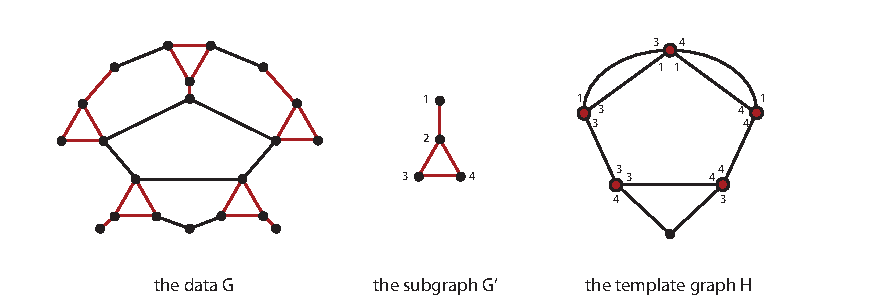
\includegraphics[width=\textwidth]{./images/illustration.pdf}
  \caption{An illustration of the motif code. We store $G'$ once, and remove it from $G$, replacing it everywhere with a single, special, node. The links to special nodes are annotated with `rewiring' information, which tells us how to rewire the subgraph back into $H$. Storing only $H$ and $G'$ is enough to reconstruct the data.}
  \label{figure:motif-code}
\end{figure*}

Assume that we are given a graph $G$, a potential motif $G'$, and a list ${\cal M} = \langle M_1, \ldots, M_k\rangle$ of sequences representing the instances of $G'$ in $G$. That is, each sequence $M\in \cal M$ consists  of nodes in $N(G)$, such that the induced subgraph $I(M, G)$ is equal to $G'$. Sequences in $\cal M$ may overlap. We are also provided with a generic graph code $L_\text{base}(G)$ on $\G$ or on $\G_\text{simple}$. 

The basic principle behind our code is illustrated in Figure~\ref{figure:motif-code}: we want to store the motif only once, remove as many instances of the motif from the data as we can, and replace them with references to the stored motif. The two graphs combined contain enough information to recover the data, but we have only had to describe the motif once. The process is described precisely in Algorithm~\ref{algorithm:motif-code}.   

The first thing we need for this scheme is a subset of $\cal M$ such that the instances contained within it do not overlap: ie for each $M_a$ and $M_b$ in the subset $M_a \cap M_b = \emptyset$. Selecting the subset that would give us optimal compression is NP-Hard (as the set cover problem is reducible to it), so we must make do with an approximation. As we will see, instances with a low number of links to nodes outside the instance are preferable. We call this the \emph{exdegree}. \footnote{Unlike the in- and outdegree the exdegree is not a property of a node, but of a subgraph.} In order to find a subset of instances with low exdegree, we first sort $\cal M$ by exdegree in ascending order. We then remove the first $M$, add it to our subset $\cal M'$ and remove all other instances that overlap with it. We continue removing the first remaining instance until $\cal M$ is empty.

In the following, we will often need to store a sequence of integers. We will store all such sequences using the code corresponding to a  \emph{Dirichlet-Multinomial} (DM) distribution. Let $S$ be a sequence with length $|S|$ and values $S_i \in [0, n_{\max}]$. Conceptually, the DM distribution models the following sampling process: we sample a probability vector $p$ on $[0, n_{\max}]$ from a Dirichlet distribution with parameter vector $\alpha$, and then sample $|S|$ symbols from the categorical distribution represented by $p$. The probability mass function corresponding to this process can be expressed as:
\begin{align*}
&\text{DirM}_\alpha(S) = \prod_{i \in [1,|S|]} \text{DirM}_\alpha(S_i\mid S_{1:i-1})  \\
&\text{DirM}_\alpha(S_i \mid S') = \frac{f(S_i, S') + \alpha_i}{|S'| + \sum_i \alpha_i}
\end{align*}
where $f(x, X)$ denotes the frequency of $x$ in $X$. We use $\alpha_i = 1/2$ for all $i$. Note that the code $- \log \text{DirM}(\cdot)$ does not include $n_{\max}$ or the length of the sequence. If these cannot be deduced by the decoder from previous parts of the code, they need to be encoded separately. Let $L_\text{DirM}(S) = -\log \text{DirM}(S)$.

We also require a self delimiting code to represent natural numbers. We will use the code corresponding to the probability distribution $p(n) = 1/ (n(n+1))$, and denote it $L_\N(n)$.

\begin{description}
\item[subgraph] First, we store the subgraph $G'$ using $L_\text{base}(G')$ bits.
\item[template] We then create \emph{template graph} $H$ by removing the nodes of each instance $M \in \cal M'$, and replacing them with a single new node called an \emph{instance node}. The internal links of $M$---those incident to two nodes both in $M$---are removed from the graph. Any link connecting a node outside of $M$ to a node inside of $M$ is kept, and rewired to the instance node.
\item[instance nodes] Which nodes of $H$ are instance nodes is not recorded by $L_\text{base}$, so we must record this separately. There are $|N_{G}| \choose |{\cal M}'|$ possibilities, so we can encode this information in $\log {|N_{G}| \choose |{\cal M}'|}$ bits.
\item[rewiring] For each side of a link in $H$ incident to an instance node, we need to know which node in the motif it originally connected to. If we assume some canonical ordering of the links in $H$, we only need to encode the sequence $W$ of integers $w_i \in [1,\ldots, n']$ with $n'=|N_{G'}|$. We do so using the DM model described above. The maximum symbol and length of $W$ can be deduced from parts already encoded. Note that this code is invariant to the ordering of $W$, so we need not specify the order in which we enumerate the links.
\item[multiple edges] If the null-model can only encode simple graphs, we cannot use it to store $H$ directly, since collapsing the instances in to single nodes may have created multiple edges. In this case we remove all multiple edges and encode them separately. We assume a canonical ordering over the links and record for each link incident to an instance node, how many copies of it were removed. This gives us a sequence $R$ of integers $r_i \in [0, r_\text{max}]$ which we store by first recording the maximum value in $L_\N(\max(R))$ bits, and then recording $R$ with the DM model.
\item[insertions] Finally, while $H$ and $G'$ give us enough information to recover a graph isomorphic to $G$, we cannot yet reproduce the specific node ordering of $G$. In order to minimize the number of bits required for this information, we first ensure that the instance nodes in the template graph always take the place of the first node of the subgraph it encodes in the node ordering. Thus, if the data is reconstructed, and the instance node is replaced by the motif, the first node of the motif takes the place of the instance node, and for the other nodes of the motif, we must specify where they should be inserted in the current node order. In this case, then we perform $n_i = |{\cal M}'| (|N_{G'}|'-1)$ such insertions. Each insertion requires $\log (t+1)$ bits to describe, where $t$ is the current size of the graph. Let $H$ be the template graph and $G$ the complete graph, then we require $\sum_{t=|N_H|}^{|N_G|-1} \log (t+1) = \log (|N_G|!) - \log (|N_H|!)$ bits to record the correct insertions.
\end{description} 

\begin{pseudo}[th]
\caption{The motif code $L_\text{motif}(G \mid G', {\cal M', L_\text{base}})$.}
\label{algorithm:motif-code}
{
Given:\\ 
\tab a graph $G$, a subgraph $G'$,\\ 
\tab a list $\cal M'$ of instances of $G'$ in $G$, a generic graph code $L_\text{base}$.\\
\\
$b \leftarrow 0$ \emph{\# the running total of bits used.} \\
$b \leftarrow b + L_\text{base}(G')$\hfill \textbf{subgraph} \\
\\
\emph{\# replace each instance with a single node} \\
$H \leftarrow \text{copy}(G)$, $W = [] $\hfill \textbf{template} \\
\textbf{for each } $M = \{ m_1, \ldots m_{|N_{G'}|}\}$ \textbf{in} $\cal M'$:\\
\tab \emph{\# We use $m_1$ (the $m_1$-th node in $G$) as the instance node}\\
\tab \textbf{for each} link $l$ between a node $n_\text{out}$ not in $M$ and a node $m_j$ in $M$:\\
\tab \tab \textbf{if} $j \neq 1$: add a link between $n_\text{out}$ and $m_j$\\
\tab \tab $W$.append$(j)$\\
\tab remove all nodes $m_i$ except $m_1$, and all incident links\\
$b \leftarrow b + L_\text{DirM}(W)\hfill\textbf{rewiring}$\\
\\
\textbf{if} $L_\text{base}$ can encode multigraphs:\\
\tab $b \leftarrow b + L_\text{base}(H)$\\ 
\textbf{else}: \hfill \textbf{multiple edges}\\
\tab $R, H' \leftarrow \text{simple}(H)$ \\
\tab $b \leftarrow b + L_\text{base}(H')$\\ 
\tab $b \leftarrow b + L_\N(\max(R)) + L_\text{DirM}(R)$\\
\\
$b \leftarrow b + \log {|N_G| \choose |{\cal M'}|}$ \hfill \textbf{instance nodes}\\
$b \leftarrow b + \log (|N_G|)! - \log (|N_H|)!$ \hfill \textbf{insertions}\\    
\\
\textbf{return} $b$\\
}
\end{pseudo}

\paragraph{search} Since our code accepts any list of motif instances, we are free to take the list $\cal M'$ and prune it further, before passing it to the motif compressor, effectively discounting instances of the motif. This can often improve compression, as instances with high exdegrees may cost more to store than we gain per motif. We will sort  $\cal M'$ by exdegree and search for the value $c$ for which compressing the graph with only the first $c$ elements of $\cal M'$ gives the lowest codelength.

The codelength $L_\text{motif}$ as a function of $c$ is roughly unimodal, which means that a ternary search should give us a good value of $c$ while reducing the number of times we have to compute the full codelength. We use a \emph{Fibonacci search} \cite{kiefer1953sequential}, an elegant variation on ternary search requiring only one sample per recursion. We provide an algorithm in the supplementary materials.

\paragraph{implementation} The \textbf{template} part of the code can be time and memory intensive for large graphs, as it involves creating a copy of the data. For any given $L_\text{base}$, we can create a specific implementation which computes the codelength required for storing the template graph without constructing $H$ explicitly. This will speed up the computation of the code at the expense of creating a new implementation for each new null model. We use such specific implementations for our three null models.

\subsection{Null models}

\subsubsection{The Erd\H{o}s-Renyi code}

The Erd\H{o}s-Renyi (ER) model is probably the most famous probability distribution on graphs\cite{renyi1959random,gilbert1959random}. It takes $n = |N_G|$ and $m = |L_G|$ as parameters, and assigns equal probability to all graphs with these attributes, and zero probability to all others. For undirected graphs, there are ${(n^2-n)/2 \choose m}$ such graphs, giving us a uniform code over this set with $\log{(n^2-n)/2 \choose m}$ bits per graph. 

In order to make this a code on $\G$ we also need to store $n$ and $m$. While this is only a small part of the code, there are many ways to do this, with no clear optimum. To show that this choice doesn't matter, we simply ignore this part of the code when using the ER model as $L_\text{null}$:
\[
L^\text{ER}_\text{null}(G) = \log{(n^2-n)/2 \choose m} \p
\] 
As explained in Section~\ref{section:model-selection}, any code that compresses better than this allows us to reject all models that are equivalent to the ER model with some choice of prior for $n$ and $m$.

When we use the ER code for $L_\text{base}$, we must make sure that it is a proper code on $\G$, so we encode $n$ with $L_\N$ and use a uniform code over the first $(n^2-n)/2$ integers for $m$. This gives us a total codelength of
\[
L^\text{ER}_\text{base}(G) = L_\N(n) + \log((n^2-n)/2) + \log{(n^2-n)/2 \choose m} \p
\]
For directed networks we have
\[
L^\text{ER}_\text{base}(G) = L_\N(n) + \log(n^2-n) + \log{(n^2-n) \choose m} \p
\]
 
\subsubsection{The degree sequence model}
\label{section:degree-sequence-model}

The most common null-model in motif analysis is the \emph{degree sequence model} (also known as the \emph{configuration model} \cite{newman2010networks}). This model takes a degree sequence $d$ as a parameter and assigns equal probability to all graphs with that degree sequence (and zero probability to all others). We will call this model $p_d$. For directed graphs, the model is parametrized by both the in-degree sequence $d^\text{in}$ and the out-degree sequence $d^\text{out}$. 

The codelength of a graph $G$ under this model, assuming that $G$ matches the degree sequence, is $\log |{\cal G}_d|$ where ${\cal G}_d$ is the set of graphs with degree sequence $d$. There is no known simple way to compute the size of this set for either directed or undirected graphs, but various estimation procedures are known. We use an importance sampling algorithm discovered independently by \cite{blitzstein2011sequential} and \cite{charo2010efficient}.\footnotemark~This algorithm is guaranteed to produce any graph matching $d$ with some nonzero probability. Crucially, the algorithm does not backtrack or reject candidates, which means that if we multiply the probability of each random choice made in sampling, we get the probability of the sample under our sampling procedure. That is, the algorithm produces, along with a sample $G$, the probability $q_d(G)$ of the algorithm producing $G$. While the samples are not uniform, we do have:
\[
{E} \left [\frac{1}{q_d(G)}\right] = |\cG_d| 
\]
where $G$ is a random variable representing a sample from the algorithm. Thus, we can sample a number of graphs and estimate the mean of their inverse probability under $q_d$ to estimate $p^d(G)$. This is a form of \emph{importance sampling}. 

\footnotetext{Specifically, our implementations uses the highly optimized algorithm described in \cite{charo2010efficient}. However the non-uniform sampling from the candidate set, discussed in \cite[p10, step 5]{blitzstein2011sequential} is crucial to achieving a low variance in the sampling distribution, and thus a fast convergence.}

Unfortunately, even with the highly optimized implementations described in \cite{charo2010efficient} and \cite{kim2012constructing} sampling can be slow for large graphs. Luckily, since we are only interested in the \emph{logarithm} of the number of graphs, we do not require a high level of accuracy. For instance, if we accept a margin of error of only 15 bits (of the potentially $10^6$ bits required to store the graph), that means we can underestimate the number of graphs by 4 orders of magnitude and still end up within the margin. All we need is a reliable confidence interval for our estimate. Our method of obtaining such a confidence interval is described in the appendix. In all cases, we use a one-sided confidence interval: when computing the codelength under the null model, we use a lower bound for the true value, and when computing the codelength for the motif code, we use an upper bound. Thus, the difference in codelength is a lower bound for the true value.

\paragraph{$L^d$ as a null-model}

In Section~\ref{section:model-selection}, we described testing against $L_{d_G}(G) = \log |{\cal G}_{d_G}|$: the degree sequence code with the correct degree sequence \emph{hardcoded}. If we found a motif that would allow better compression than $L_{d_G}$, we could conclude that no property of the degree sequence can explain the prevalence of the motif. 

However, at the size of graph for which the degree-sequence model is currently tractable---those graphs tested in Section~\ref{section:various}---the data does not provide enough evidence for such a claim. Instead, we choose another model that dominates a large subset of models based on the degree sequence.

For this model, we make one additional assumption: that the degrees are independently distributed. In coding terms, this simply means that we have some code $L_\pi$ on the integers, which is used to store the degrees one by one. No such code can compress the degree sequence better than the one which uses the frequency $f^d_i$ with which each integer $i$ actually occurs in $d$. This gives us the following null model
\[
L^f_\text{null}(G) = |d| \log |d| - \sum_{i \in \{1, \ldots, |d|\}} \log f^d_{d_i} + \log |\G_d| \p  
\] 
With this null model can still reject, for instance, the null hypothesis that the degrees originate from a power law distribution. That is, if the power law distribution of $d$ were the only structural property of the graph, we should not be able to find a motif with which we can compress significantly better than $L^f_\text{null}$.

We will estimate the last term of this code using a one-sided confidence interval at $\alpha=0.05$ to get a lower-bound of the true value. 

\paragraph{$L^d$ as a base model} For $L^d_\text{base}$ we need a code on $\G$. First, we store the size of the graph with $L_\N$. We then store the maximum degree and encode the degree sequence with the DM model:
\[
L^d_\text{base}(G) = L_\N(|N_G|) + L_\N(\max(d)) + L_\text{DirM}(d) + \log |\cG_d|  
\]
Now, when we use this base in $L_\text{motif}$, the intractable value $|\cG_d|$ occurs in two places: the encoding of the subgraph, and the encoding of the template graph. Since we use our estimator for both, we must be careful to end up with a correct confidence interval for the resulting motif code. Let $d'$ be the degree sequence of the subgraph, and $d$ be the degree sequence of the template. Then, we can split the total code length into three components: $\log |\cG_{d'}|$, $\log |\cG_d|$ and $R$. $R$ is the sum of all parts of the code that we can compute exactly, including the sizes and sequences of the motif and template graph (ie. everything but $\log |\cG_{d'}|$ and $\log |\cG_d|$). The total codelength is described by $\log |\cG_{d'}| + \log |\cG_d| + R$, where the first two terms require the use of the estimator. Let $Q_m$ and $Q_h$ be random variables representing the inverse probability of graphs sampled from the importance sampling algorithm, for the degree sequence of the motif and the template graph respectively. In other words, the true codelength for the motif code is:
\begin{align*}
& \log E Q_m + \log  E Q_c + R \\ 
= & \log E Q_m E Q_c + R \\
= & \log E [Q_m Q_c] + R
\end{align*}
where the last line follows from the fact $Q_m$ and $Q_c$ are independent. So to get a correct confidence interval, we can take the same number of samples of both $Q_m$ and $Q_c$, multiply their probabilities, and perform the bootstrap analysis on the list of these multiplied probabilities (since we are summing the logarithms of log-normally distributed variables, the result is log-normally distributed as well). 
For $L_\text{base}^d$, we compute a one-sided confidence interval to get an \emph{upper}bound, so that with 95\% confidence we are \emph{over}estimating the size of the motif code. 

\subsubsection{The edgelist model}

While estimating $|\cG_d|$ can be costly, we can compute an upper bound efficiently. Assume that we have a directed graph $G$ with $n$ nodes, $m$ links and a pair of degree sequences $d = (d^\text{in}, d^\text{out})$. To describe $G$, we might write down the links as a pair of sequences $(F, T)$ of nodes: with  $F_i$ containing the node from which link $i$ originates, and $T_i$ containing the node to which it points. Let $S_d$ be the set of all pairs of such sequences satisfying $d$. We have $ m \choose d_1^\text{in}, \ldots, d_n^\text{in}$ possibilities for the first sequence, and $m \choose d_1^\text{out}, \ldots, d_n^\text{out}$ for the second. This gives us $|S_d| = {m \choose d_1^\text{in}, \ldots, d_n^\text{in}}{m \choose d_1^\text{out}, \ldots, d_n^\text{out}} = m!m! / \prod_{i=1}^n d^\text{in}_i ! d^\text{out}_i !$. We have $|S_d| > |\cG_d|$ for two reasons. First, many of the graphs represented by such a sequence pair contain multiple loops and self-loops. Second, the link order is arbitrary: we can interchange any two different links, and we would get a different pair of sequences, representing the same graph. 

To find our upper bound, let $S'_d \subset S_d$ be the set of sequence pairs representing simple graphs. Since all links in such graphs are distinct, we have $|\cG_d| = |S'_d|/m!$. Since $|S'_d| \leq |S_d|$, we have \footnotemark
\[
|\cG_d| \leq \frac{m!}{\prod_{i=1}^n d^\text{in}_i ! d^\text{out}_i !} \p
\]

\footnotetext{This value was previously used in \cite{bezakova2006graph} as a precise value for the number of graphs with multiple edges. This is incorrect, as we can only divide by $m!$ if we know that no graphs have multiple edges.}

In the undirected case, we can again describe the graph as a pair of sequences of integers, where the direction of the link is ignored. As before, we define $S_d$ as the set of all such pairs satisfying $d$. We now have an additional reason why $S_d > |\cG_d|$: each pair of nodes describing a link can be swapped around to give us the exact same graph. This gives us:
\[
|\cG_d| \leq |S'_d| / (2^m m!) = \frac{m!}{2^m \prod_{i=1}^n d_i! d_i!} \p
\]

In both cases, the fact that we have an upperbound gives us a code: while the code as described assigns some probability mass to non-simple graphs, we can easily assume that this is assigned instead to some null-element, since we are only interested in the codelengths and probabilites of simple graphs. This gives us the following basic codelength for directed graphs:
\[
L^\text{EL}(G) = \log m! - \sum_{i=0}^n \log d_i^\text{in}! - \sum_{i=0}^n \log d_i^\text{out}!   
\]
where $(d^\text{in}, d^\text{out})$ are the degree sequences of $G$. and for the undirected case:
\[
L^\text{EL}(G) = \log m! - m - \sum_{i=0}^n 2 \log d_i! \p   
\]

As with the degree-sequence model, we also need to store the degree sequences themselves. We use the same technique: for the null models we use the frequencies from the sequence itself, and for the base models, we use $L_\N$ for the size, and $L_\text{DirM}$ for the degree sequence. 

\section{Experiments}

To validate and illustrate our method, we will perform three experiments. First, we will construct a synthetic network, by enriching a random network with a single motif. The method should recover only this motif as significant. Second, we will run the method on datasets from four different domains, and show the results for the most frequent subgraphs, using the three null-models we have described. Finally, to show the scalability of the model, so long as fast null models are used, we will run the analysis on a large graph.

In all experiments we search for motifs by sampling, based on the method described in \cite{kashtan2004efficient}. Note that we have no particular need for a sampling algorithm which provides an accurate approximation of the actual frequencies present in the graph, so long as it can provide us with a large selection of non-overlapping instances with low exdegree. For this reason we adapt the algorithm to improve its speed: we start with an empty selection of nodes $N'$, and add a random node drawn uniformly. We then add to $N'$ a random neighbour of a random member of $N§$, and repeat this action until $N'$ has the required size. We then extract and return $I(N', G)$. In the case of a directed graph both nodes reachable by in- and by outdegrees are considered neighbours.  

The size $|N_G'|$ of the subgraph is chosen before each sample from a uniform distribution over the interval $(n_\text{min}, \text{max})$.

We re-order the nodes of the extracted graph to a canonical ordering for its isomorphism class, using the Nauty algorithm \cite{mckay1981practical}. We maintain a map from these isomorphic subgraphs to a list of instances found. After sampling is completed, we end up with a set of potential motifs and a list of instances for each, to pass to the motif code described in Section~\ref{section:motif-code}.

In all cases we report the log-factor, which is equal to the difference in bits between the graph compressed with the null model and the graph compressed using the motif model. If the log-factor is larger than 10 bits, we can interpret it, as described in Section~\ref{section:model-selection} as a successful significance test, allowing us to reject the null model at $\alpha=0.001$. In the case of the degree-sequence model, we actually report a lower-bound to the factor as described in Section~\ref{section:degree-sequence-model}. In all cases, a negative factor means that we do not have sufficient evidence to reject the null-model, but a different experiment might yet achieve a positive log-factor. This could be achieved by: sampling more subgraphs, using a different algorithm to find motif instances or taking more samples from the degree-sequence estimator.

\subsection{Recovering motifs in synthetic data}

\label{section:recovering}

\begin{figure*}[h]
  \hspace{-4cm}
  \includegraphics[width=20cm]{./images/synthetic-plot.pdf}
  \caption{\small The results of the experiment on synthetic data. The bottom row shows all 21 simple connected graphs with 5 nodes (up to isomorphism). The middle row shows the frequencies for $n^i = 0$, $n^i=10$ and $n^i=100$ from left to right, for each motif. The bars show the average value over 10 randomly sampled graphs, with the same subgraph (shown in red) injected each time. The top row shows the difference between  the code length under the null model (the ER model) and under the motif code. The error bars show the \emph{range} of the data.}
  \label{figure:plot-synthetic}
\end{figure*}

We use the following procedure to sample an undirected graph with $5000$ nodes and $10000$ links, containing $n^i$ injected instances of a particular motif $G'$ with $n'$ nodes and $m'$ links:

\begin{enumerate}
  \item Let $n = 5000 - (n'-1)n^i$ and $m = 10000 - m'n^i$ and sample a graph $H$ from the uniform distribution over all graphs with $n$ nodes and $m$ links.   
  \item Label $n^i$ random nodes, with degree 5 or less, as instance nodes.
  \item Let $p_v$ be a categorical distribution on ${1, \ldots, 5}$, chosen randomly from the uniform distribution over all such distributions.
  \item Label each place an edge connects to an instance node with a random integer from $p_v$.
  \item Reconstruct the graph $G$ from $G'$ and $H$.
\end{enumerate}

This is roughly similar to the process of sampling from our motif code. If our assumptions are correct, and we choose $n^i$ high enough, $G'$ should be the only significant subgraph in $G$, with the exception of motifs that can be explained from the prevalence of $G'$, ie. subgraphs and supergraphs of $G'$, or graphs that contain part of $G'$. However, these should have a markedly lower factor than $G'$. For our experiment, we will only extract subgraphs of size 5, to rule out the first two cases.

On this sampled graph, we run our motif analysis. We run the experiment three times, with $n^i = 0$, $n^i = 10$ and $n^i = 100$, using the same subgraph $G'$ over all runs, but sampling a different $H$ each time. Per run we sample 5000 motifs. Note that this  sample size is not chosen for performance reasons; we aim to show that a very \emph{low} sample size is sufficient to recover the motif. The null-model in all cases is the ER model, as that corresponds to the source of the data.

Figure~\ref{figure:plot-synthetic} shows the results for the 21 possible connected subgraphs of size 5. As expected, when we insert no subgraphs, the motif code cannot compress the graph better than the motif model, for any motifs, since the source of the data \emph{is} the null-model. There are motifs with very high frequencies (shown on the right), much higher than the frequencies of our motif, but these are a consequence of the null model and have a negative log-factor. We can also see that once we insert 100 instances of the motif, two other subgraphs become motifs: in both cases, these share a part of the inserted motif (a rectangle and a triangle). This is an important lesson for motif analysis: not every motif represents a meaningful result, some motifs may be the result of the presence of other motifs. 

\subsection{Various datasets and null models}
\label{section:various}

Next, we show how our our approach operates on a selection of datasets across domains. We use the following datasets:
\begin{description}

\item[kingjames (undirected, $n=1773, m=9131$)] Co-occurrences of nouns in the text of the King James bible \cite{konect:2014:moreno_names,konect:harrison}. Nodes represent nouns (places and names) and links represent whether these occur together in one or more verses.
\item[yeast (undirected, $n=1528, m=2844$)] A network of the protein interactions in yeast, based on a literature review \cite{reguly2006comprehensive}. Nodes are proteins, and links are reported interactions between proteins. we removed 81 self-loops from the network.
\item[physicians (directed, $n=241, m=1098$)] Nodes are physicians in Illinois \cite{konect:2015:moreno_innovation,konect:coleman1957}. Links ondicate that one physician turns to the other for advice.
\item[citations (directed, $n=1769, m=4222$)] The arXiv citation network in the category of theoretical astrophysics, as released for the 2003 KDD Cup \cite{gehrke2003overview}. To create a workable graph, we follow the procedure outlined in \cite{carstens2013motifs}: we include only papers published before 1994, remove citations to papers published after the citing paper, and select the largest connected component.
\end{description}

All datasets are simple (no multiple edges, no self-loops). In each case we take $5 \cdot 10^6$ samples with $n_\text{min} = 2$ and $n_\text{max} = 6$. We test the 50 motifs with the highest number of instances (after motif removal), and report the log-factor for each null model. For the edgelist and ER models we use a Fibonacci search at full depth, for the degree-sequence model we set the search depth to $3$. For the degree-sequence estimator, we use 20 samples and $\alpha=0.05$ to determine our confidence interval. For each motif, with the same set of instances, we use the three different null-models described to compress the data, and report the log-factor.   

\begin{figure*}[p]
  \includegraphics[width=\textwidth]{./images/kingjames/compare-plot.pdf}\\
  \includegraphics[width=\textwidth]{./images/yeast/compare-plot.pdf}\\
  \caption{The results of the motif extraction on the 2 undirected networks.}
  \label{figure:plot-und}
\end{figure*}
  
\begin{figure*}[p]
  \includegraphics[width=\textwidth]{./images/physicians/compare-plot.pdf}\\
  \includegraphics[width=\textwidth]{./images/citations/compare-plot.pdf}\\
  \caption{The results of the motif extraction on the 2 directed networks.}
  \label{figure:plot-dir}
\end{figure*}

Our first observation is that for the physician dataset, there are no motifs under the degree-sequence null-model. We've found this to be a common property of many social networks. Whether this indicates that social networks are simpler, more random, or perhaps even well-modeled by the degree sequence model, requires further investigation. 

In both the \emph{kingjames} and the yeast \emph{datasets}, many motif contain cliques or near-cliques. This suggests that the data contains local communities of highly connected nodes which the null model cannot explain.

We also observe the reasonable agreement between the degree sequence model and the edgelist model, suggesting that the edgelist model can be an acceptable proxy for the degree sequence model. 

\subsection{Large-scale motif extraction}
\label{section:large}
In order to test the scalability of the method for null-models which are easy to compute, we forgo the degree-sequence model and test the approach on the hyperlink graph of the Dutch Wikipedia \cite{konect:2015:link-dynamic-nlwiki,konect:unlink}. This dataset contains all links that existed at some point between two articles in the Dutch Wikipedia. We removed self loops and multiple edges, resulting in a network of 1 039 253 nodes and 13 485 902 links.  We sampled $5 \cdot 10^6$ subgraphs of sizes from 2 to 6 nodes. We selected the 100 motifs with the greatest number of instances (after overlap removal), and ranked these by the log-factor of the edgelist model. The top 20 are shown in Figure~\ref{figure:plot-large}. We used the Fibonacci search at full depth.

The analysis was executed using 3.5 gigabytes of Java heapspace, on a machine with an 1.80 Ghz Intel Xeon processor (E5-2650L). It took 5 hours and 27 minutes to complete. Sampling of subgraphs took 9 minutes, overlap removal took 14 minutes and the compression analysis took, on average, 3 minutes and 2 seconds per motif (for 100 motifs analyzed).

Note that all code in this analysis is single-threaded, so the availability of multiple cores was not exploited.

\begin{figure*}[htb]
  \hspace{-4cm}
  \includegraphics[width=20cm]{./images/large/compare-plot.pdf}
  \caption{The results of the motif extraction on a large-scale network. We show the thirty motifs with the highest log-factor under the EL model.}
  \label{figure:plot-large}
\end{figure*}

\section{Conclusion} 

We have  introduced a new, fast method of testing motif relevance, based on MDL principles. We have shown that this method allows motif analysis to be scaled up to graphs with millions of nodes, even on commodity hardware. 

One thing shown in our experiments deserves further mention: in Section~\ref{section:recovering}, we saw that injection of one subgraph into a network could cause other subgraphs to become motifs (ie. statistically significant). This tells us that even \emph{if} some motifs represent functional units of a network, as is often claimed (and contested) \cite{milo2002network,konagurthu2008origin}, the fact that a subgraph occurs with statistically significant regularity cannot be taken as proof this fact, even if we assume that the null model is perfectly chosen. The use of hypothesis testing is a misleading factor here. Hypothesis testing allows one to make a binary decision, but that decision is always \emph{about the null-model}. A sufficiently low $p$-value should not be construed as evidence that a subgraph is a functional unit in the network. In fact, at this level of abstraction, the best any method can do is to offer sound candidates for functional units. The \emph{proof} that a particular motif actually corresponds to a meaningful unit can only be achieved in context: that is, a domain expert should evaluate the list of instances found for a particular motif, to see whether a large subset of them perform the same role in the network, or if not, what other reason can be found for the prevalence of the motif. In summary, it is important to keep in mind that motif analysis is necessarily an \emph{exploratory} technique, and while a significance test provides a good heuristic to separate trivially frequent subgraphs, from subgraphs which may represent important properties, it is ultimately just a heuristic. The only thing it \emph{proves} is the incorrectness of the null-model. 

The reader may note that while we have shown that our method is fast in principle, if we wish to use the degree-sequence model, we are still limited to medium-scale graphs, and long processing times. This is true, but there are several potential ways around this problem. First, $L^d_\text{null}(G)$ only needs to be computed once for each $G$. After that, any MDL or Bayesian analysis (for motifs, cliques, clustering, etc.) can make use of this same value. Second, while we have chosen to use the null model as $L_\text{base}$, to ensure that our compression could only be caused by the frequency of the motif, this is not the only approach. We could also use the edgelist model as $L_\text{base}$: since the edgelist code upperbounds the degree-sequence model, any positive log-factor in this setting means we would also get a positive log-factor with the degree sequence model as $L_\text{base}$. Our second option is to find a null-model that can be computed quickly, but which \emph{dominates} the degree-sequence model. As noted in Section~\ref{section:model-selection}, any subgraph that is a motif under such a model is also a motif under the degree-sequence model. 


One drawback to our approach is that we cannot currently offer a simple way to detect anti-motifs. Technically, the fact that a given subgraph occurs much less than expected under a null model, should allow us to compress the graph: any non-randomness can theoretically be used to compress a graph. However, we do not see a straightforward way in which such a code could be made practical. 

Finally, we hope that our approach is illustrative of the general benefit of MDL techniques in the analysis of complex graphs. Conventional methods often require us to match an observed property to a model described in terms of a process generating the graph. The MDL principle allows us to  bridge these two approaches. Instead of seeing probability distributions as random processes producing graphs, we can see them as descriptions of graphs. The trick then, is not to find a process that produces graphs with the desired property, but to find a description method that is efficient for graphs with the desired property. For many properties (large cliques, motifs, degree sequences) such a description method readily suggests itself. 

\section{Appendix: Confidence intervals for the degree-sequence model}
\label{section:confidence-intervals}

In \cite{blitzstein2011sequential}, the sample mean $1/n \sum_i 1/q(G_i)$ is used as an estimator for the required expectation. However, as shown in \cite{charo2010efficient}, the distribution of $1/q(G_i)$ tends to be very close to log-normal. This means that the sample mean will converge \emph{very} slowly to the correct value. For instance, a log-normal distribution with $\mu=200$ and $\sigma=10$ will have an arithmetic mean of  $e^{250}$, yet the sample mean after as much as $10^6$ samples, will almost always be around $e^{235}$. Clearly, this estimator is unreliable for practical sample sizes.

For this reason, we instead use the \emph{maximum likelihood estimator} for the log normal distribution. Let $Q_i = 1/q_d(G_i)$. We assume $Q_i$ is log-normally distributed, so that $Y_i = \log Q_i$ is normally distributed. Let $\overline{Y} = 1/n\sum_i Y_i$ and $S_Y = 1/n \sum_i (\overline{Y} - Y_i)^2$; then the maximum likelihood estimator of $EQ$ is $\exp\left(\overline{Y} + \frac{1}{2}S_Y\right)$. Thus, the codelength under the degree sequence model can be estimated as $\left(\overline{Y} + \frac{1}{2}S_Y\right)\log_2(e)$.

As mentioned in the body of the text, even with the highly optimized implementations described in \cite{charo2010efficient} and \cite{kim2012constructing} sampling can be slow for large graphs. In our implementation, a modern day laptop can take several minutes to produce a single sample for a random graph with $10^4$ nodes and $10^5$ links. Luckily, since we are only interested in the \emph{logarithm} of the number of graphs, we do not require a high level of accuracy. For instance, if we accept a margin of error of only 15 bits (of the potentially $10^6$ bits required to store the graph), that means we can underestimate the number of graphs by 4 orders of magnitude and still end up within the margin. All we need is a reliable confidence interval for our estimate. If we have that, we can take the lowerbound of the confidence interval as the codelength of our null model, and be confident that we are erring on the side of caution. If the motif model does better than the lowerbound of the confidence interval, we can reject the null model with confidence.

Since we are dealing with a log-normal source, we cannot simply use twice the standard error of the means to approximate our error bars. We will use the parametric bootstrap procedure provided in \cite{angus1994bootstrap,zhou1997confidence}. To substantiate this method, we test the coverage of the two-sided symmetric confidence interval on three datasets. We proceed as follows: first we estimate the true value of $|\cG_d|$ with the ML estimator, using $10^6$ samples. Call this value $g$. We use this as our gold standard. We then sample a small number (5, 10, 20) of graphs and their associated probabilities. Using the bootstrap method we construct a two-sided symmetric confidence interval with $\alpha = 0.05$ on this sample. We repeat the procedure of sampling data and constructing an interval 5000 times and report the number of times $g$ was inside the confidence interval. If the bootstrap method is accurate the resulting value should be close to 0.95. We use the following datasets:
  \begin{description}
  \item[cattle] Observed dominance behaviors between cows. A directed graph with 28 nodes, and 217 links. \cite{schein1955social,konect:2015:moreno_cattle}
  \item[revolution] Affiliations of 136 people to 5 organizations encoded as a bipartite graph. 141 nodes and 160 links. \cite{konect:2015:brunson_revolution}
  \item[random] A simple undirected random graph of 50 nodes, each pair of distinct nodes connected with probability $0.5$.
  \end{description}
As Table~\ref{table:coverage-experiment} shows, this method becomes relatively reliable at around 10 samples, although the intervals are quite large at that sample size.

\begin{table}
  {\centering
  \begin{tabular}{|r|r r|r r|r r|}
  \hline
   &  \multicolumn{2}{c|}{5 samples} & \multicolumn{2}{c|}{10 samples}  & \multicolumn{2}{c|}{20 samples}  \\
  cattle  & 0.93 & 511 (379) & 0.94 & 194 (94.6) & 0.94 & 107 (35.3) \\
  revolution   & 0.89 & 147 (120) & 0.92 & 59.3 (29.2) & 0.93 & 33.5 (11.3) \\
  random  & 0.91 & 108 (97.0) & 0.94 & 44.7 (24.5) & 0.94 & 25.3 (9.44) \\
  \hline
  \end{tabular}
  }

  \caption{Coverage and interval length at $\alpha=0.05$ for three small datasets. The coverage is the number of times the true value $g$ was contained in the interval, over 5000 trials. The length is the mean length of these intervals in bits. The standard deviation is given in parentheses. } 
  \label{table:coverage-experiment}
\end{table}